\documentclass[11pt]{article} 



\makeatletter
\renewcommand\section{\@startsection{section}{1}{\z@}%
                                  {-3.5ex \@plus -1ex \@minus -.2ex}%
                                  {2.3ex \@plus.2ex}%
                                  {\normalfont\large\bfseries}}
\makeatother

\addtolength{\oddsidemargin}{-.875in}
\addtolength{\evensidemargin}{-.875in}
\addtolength{\textwidth}{1.75in}
\addtolength{\topmargin}{-.875in}
\addtolength{\textheight}{1.75in}


\usepackage{amssymb}
\usepackage{amsmath}
\usepackage{amsthm}
\usepackage{graphicx,caption,subcaption}


\usepackage{titling}
\setlength{\droptitle}{-6em}
\posttitle{\par\end{center}\vspace{-4.8em}}

\newcommand{\R}{{\ensuremath{\mathbb{R}}} }
\newcommand{\Q}{{\ensuremath{\mathbb{Q}}} }
\newcommand{\C}{{\ensuremath{\mathbb{C}}} }
\newcommand{\N}{{\ensuremath{\mathbb{N}}} }
\newcommand{\Z}{{\ensuremath{\mathbb{Z}}} }

\newcommand{\sexion}{\addtocounter{section}{1} }


\newcommand{\hint}[1]{{(\emph{Hint:} #1)}} %This line shows hints
%\newcommand{\hint}[1]{} %Use this line to hide all hints


\usepackage{fancyhdr}
\pagestyle{fancyplain}
\renewcommand{\headrulewidth}{0pt}

\begin{document}

%\lhead{}
\rhead{Example}
\section{Problem/Solution}
\[ y' = A y \quad\quad\quad A = \left( \begin{matrix} 2 & -4 \\ 8 & -6 \end{matrix} \right) \]
First compute 
\[\mathrm{Trace}(A) = 2- 6 = -4 \quad det(A) = (2 \cdot -6) - (-4 \cdot8) = -12 +32 = 20 .\]
Thus, the characteristic polynomial is given by 
\[\lambda^2 +4 \lambda +20,\]
and the eigenvalues are 
\[ \lambda = \frac{-4 \pm \sqrt{16 - 4 \cdot 20}}{2} = -2 \pm 4 i.\]
Let's choose to work with $\lambda = -2 +4i$. We know that the solution is $y(t) = e^{\lambda t} v$ for $v$ the associated eigenvector, so we need to find $v$. Let $v = (a~b)^T$.
\[A v = \lambda v \Rightarrow 2 a - 4 b = (-2 +4 i) a \Rightarrow (4 -4 i ) a = 4 b \Rightarrow (1 - i) a = b.\]
So, we conclude that $v = (1~1-i)^T$ is an eigenvector corresponding to $v$.


Solutions are therefore (plugging in to above)
\[y(t)= e^{(-2 +4i)t}\left( \begin{matrix}1 \\ 1-i\end{matrix}\right).\]
But we don't like complex numbers, so let's separate this into real/complex parts.
\[y(t) =  e^{(-2 +4i)t}\left( \begin{matrix}1 \\ 1-i\end{matrix}\right) =e^{-2t} (\cos(4t) + i  \sin(4t)) \left[ \left( \begin{matrix}1 \\ 1\end{matrix}\right) + i \left( \begin{matrix}0 \\ -1\end{matrix}\right) \right], \]
so
\[y_1(t) = \Re (y (t)) = e^{-2t} \left(\cos(4t)   \left( \begin{matrix}1 \\ 1\end{matrix}\right) +   \sin(4t) \left( \begin{matrix}0 \\ 1\end{matrix}\right) \right), \]
\[y_2(t) = \Im (y (t)) = e^{-2t} \left(\sin(4t)   \left( \begin{matrix}1 \\ 1\end{matrix}\right) -   \cos(4t) \left( \begin{matrix}0 \\ 1\end{matrix}\right) \right), \]

\section{Analysis}
Here's a plot of some solutions:
\[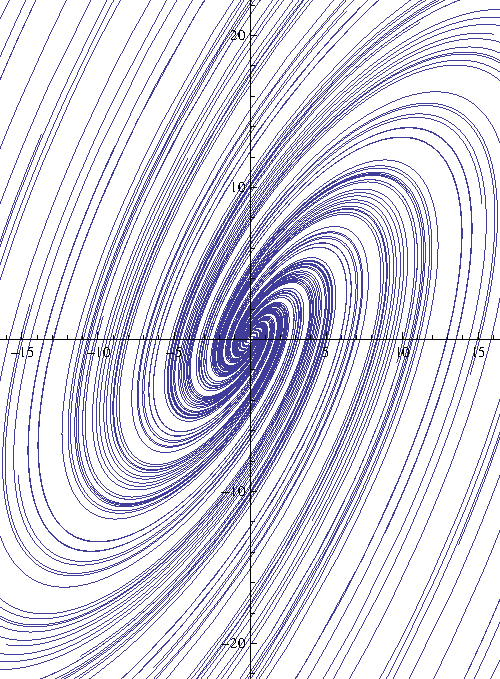
\includegraphics{plot}\]

Observe that
\[y_1(t- \pi/8) = \left(\begin{array}{c} e^{\frac{\pi }{4}-2 t} \sin(4 t) \\ e^{\frac{\pi }{4}-2 t} (-\cos(4 t)+\sin(4 t))\end{array}\right) = e^{\pi/4} e^{-2t} \left(\begin{array}{c}  \sin(4 t) \\ -\cos(4 t)+\sin(4 t)\end{array}\right) = e^{\pi / 4} \cdot y_2(t) \]
so, in fact, any curve that we can write as a multiple of $y_1$ can also be written as a multiple of $y_2$, albeit for a different range of $t$. 

This is why if we just want to know what the plane looks like, we can work with just one of $y_1, y_2$. However, if we want to solve some IVP, say $y(0) = (a~b)^T$, then we need both.

\begin{align*}a y_1(0) + b y_2(0) &= a e^{-2t} \left(\cos(4t)   \left( \begin{matrix}1 \\ 1\end{matrix}\right) +   \sin(4t) \left( \begin{matrix}0 \\ 1\end{matrix}\right) \right)+ b  e^{-2t} \left(\sin(4t)   \left( \begin{matrix}1 \\ 1\end{matrix}\right) -   \cos(4t) \left( \begin{matrix}0 \\ 1\end{matrix}\right) \right)\\
&= a    \left( \begin{matrix}1 \\ 1\end{matrix}\right) - b  \left( \begin{matrix}0 \\ 1\end{matrix}\right) 
\end{align*}
So, we can only handle initial conditions of the form $y(0) = (a~a)^T$ with $y_1$, and $y(0) = (0~b)$ with $y_2$.

\begin{figure}
        \centering
        \begin{subfigure}[b]{0.45\textwidth}
                \centering
                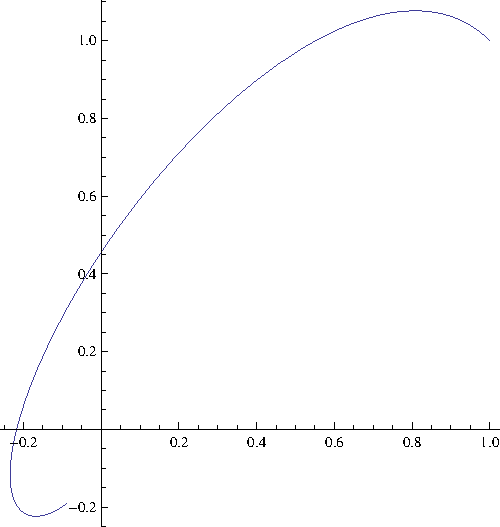
\includegraphics[width=\textwidth]{curve}
                \caption{$y_1(t), 0 \leq t \leq 1$}
        \end{subfigure}%
        ~ %add desired spacing between images, e. g. ~, \quad, \qquad etc. 
          %(or a blank line to force the subfigure onto a new line)
        \begin{subfigure}[b]{0.45\textwidth}
                \centering
                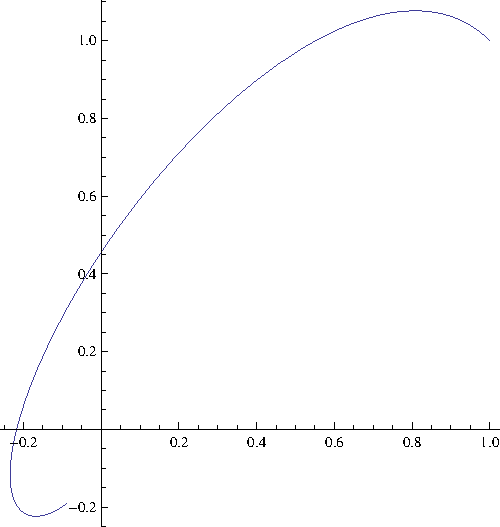
\includegraphics[width=\textwidth]{curve}
                \caption{$ e^{\pi /4} \cdot y_2 , \frac{\pi }{8}\leq t \leq 1+\frac{\pi }{8} $}
        \end{subfigure}
\end{figure}



\end{document}
